\chapter{Cryptography Fundamentals}

\section{Definition}

In present and past it is and always has been important for messages to be
transmitted securely and without the danger of information disclosure.  To meet
these requirements, two main technique have emerged:

One technique is called steganography. This discipline focuses on hiding the
transmission of messages. An example for this can be found in the past: To hide
a message, one used to shave off all hairs of a messenger. Then, the message
was tattooed on the skin. After a while, when the hair grew back, the messenger
was sent to the receiver. Border controls didn't notice this kind of message
transmission at the beginning, but after a while, the controls were informed to
check if a person was transmitting that kind of message. It was genious to
covertly transmit a message, but as soon as the message was discovered, the
information was disclosed. As a result, the message itself should have some
protection, so that only the desired receiver could read it. This was the point
in time when cryptography was born.

Cryptography is the art of encrypting a message so that only receivers with
specific knowledge can obtain the plaintext. The first steps in cryptography
were simple so called substitution ciphers, when some symbols in an alphabet
were switched or rotated.

Imagine the following message:

\vspace{0.5cm}
\textit{attack at dawn}
\vspace{0.5cm}

If one substituted all "a"s with a "z" and all "t"s with an "e", the message
would look like this:

\vspace{0.5cm}
\textit{zeezck ze dzwn}
\vspace{0.5cm}

The message immediately becomes unreadable for someone who doesn't know about
the underlying subsitution. This was, when cryptanalysis comes in: If one looks
at the text, one could for example analyze the frequency of some specific
letters, in this example "z" and "e". The most common letters in the English
alphabet are "e" and "a". One could now try to substitute the letter "z" with
"e". The outcome would be

\vspace{0.5cm}
\textit{aeeack ae dawn}
\vspace{0.5cm}

If one can't guess that the message is \textit{attack at dawn}, one could
continue using cryptanalysis. Since substituting "e" with commonly used letters
fails, one could analyze two letter chains. One of the most common used two
letter combinations with "a" is "at" (as one could have guessed when seeing
"ae").  After substituting "e" with "t", the original message is revealed.

\vspace{0.5cm}
\textit{attack at dawn}
\vspace{0.5cm}

Soon, this procedure also became quite insecure and cryptographers tried to
find new ways to encrypt their messages. It was a gift for them when computers
became commonly available: Procedures requiring masses of mathematical
operations could be executed in less than a second, complex encryption
algorithms appeared.

In modern cryptography there are two main kinds of encrypting and decrypting a
message. The first kind (which was actually also the first one that emerged) is
called \textit{symmetric encryption}. This kind of cryptography uses the same
key for en- and decryption of a message. The previously mentioned substitution
cipher is a \textit{symmetric encryption}, where the substitution table is the
key which is used for en- and decryption.

The other encryption kind is called \textit{asymmetric encryption}. Here, en-
and decryption are seen as different operations. That's why one has to use an
encryption and a decryption key to perform \textit{asymmetric encryption}.

\section{Cryptographic primitives}

The most basic building blocks in the field of cryptography are known as
cryptographic primitives. They include well researched, reliable and accepted
algorithms. Digital signatures, one-way has functions, as and public key
cryptography are examples for cryptographic primitives.

\subsection{Prime numbers}

Prime numbers are natural numbers which are greater than one and only evenly
divisible by one and themselves.

Those numbers play a main role in cryptography as they are commonly used
as a security factor. For example, it is quite difficult to determine the
prime factorization of a number, as none of the existing algorithms solves
the problem in polynomial time. Therefore, prime factorization is a problem
of \textit{nondeterministic polynomial time complexity} and to factorize
large numbers, more time than the age of the universe is needed.

But how can one get prime numbers in a short amount of time? There are two
main known solutions: The first solution is to permute through all positive
natural numbers, more efficient algorithms here are for example the
\textit{Sieve of Erathostenes} or the \textit{Sieve of Atkin}. The other
main approach is the statistical or heuristic approach. Well known methods
here are the \textit{Miller Rabin Test}, a test which delivers the propability
of a number to be a prime or not. This test is used in \textit{OpenSSL} to
find large primes, which makes it possible for users of \textit{OpenSSL} to
not have primes as factors of their RSA modulus.

\subsection{RSA}
	
RSA is an asymmetric encryption standard, developed by Rivest, Shamir and
Adleman. As many other asymmetric encryptions, RSA uses a one way function
with a trapdoor. So in order to understand RSA, one has to understand the
trapdoor function. The RSA trapdoor function relies on Euler's totient function
$\phi$. This function returns the amount of numbers, which are relatively prime
and smaller than a number n. Since prime numbers are only evenly divisible by
1 and themselves, the totient function returns n - 1 for prime numbers. Also,
if you multiply a number with another, the totient function also mutliplies
with the totient function of the other number. An example:

$$\phi(13) = 12$$

$$\phi(11) = 10$$

$$13 * 11 = 143$$

$$\phi(143) = \phi(13) * \phi(11) = 120$$

RSA uses this as follows: To encrypt something, one needs the so called
public key. To decrypt something, one needs the private key. Both keys
contain the so called RSA modulus \textit{n}, which is the product of 
two primes, \textit{p} and \textit{q}. The public key additionally has
the number \textit{e} and the private key has the additional number
\textit{d}. \textit{e} is a number which is coprime to the result of
the totient function of \textit{n}. \textit{d} is the multiplicative inverse
\footnote{The multiplicative inverse of a number a is the number b where $a*b = 1$} of
\textit{e} relative to $\phi(n)$.

Having calculated those needed factors, it is easy to en- and decrypt
a message representative (usually a number). To encrypt a message, one
has to apply the following procedure:

$$c = m^e mod N$$

Where \textit{c} is the ciphertext and \textit{m} the message representative.

The decryption follows the same procedure, only \textit{c} and \textit{d} are
swapped and the exponent is \textit{d}:

$$m = c^d mod N$$

Using this procedure without further additions isn't considered safe today:
One plaintext would always produce the same ciphertext. This is why cryptographers
started to use \textit{paddings}. Paddings wrap the plaintext and the padded
text is then encrypted. After decryption, the padding has to be removed in order
to obtain the original plaintext. As a result, to en- and decrypt a message, one
has to know the RSA procedure as well as the used padding.

\section{Cryptographic Protocols}

A cryptographic protocol is a combination of cryptographic primitives,
algorithms and possibly other cryptographic protocols. The protocol describes
how the cryptographic algorithms are used in order to increase confidentiality,
integrity and availablility of the underlying goal.

Cryptographic protocols are usually defined abstract in order to leave language
specific dificulties up to the implementation. Since only the interfaces are
defined, the developers can implement against those and therefore make sure
different implementations are compatible to each other.

\subsection{Diffie Hellmann}

\section{Secret Sharing}

Describe simple secret sharing (every participant needs all shares to
reconstruct the secret)

\subsection{Shamir's Secret Sharing}
\subsection{Blakley's scheme}

\chapter{Duse}
\section{The Cryptographic Protocol}

The protocol involves a server and a client. During a secrets lifecycle, there
are four events that are relevant for the protocol creating, reading, updating,
and deleting. These are also known as \textit{CRUD}.

\subsection{Creating a secret}

When creating a secret, the client first has to retrieve all profiles of the
users the secret should be shared with. These profiles contain the public key
of each user.

Now shamir's secret sharing could be used to split the secret into shares for
each user, however, this can lead to problems. Since shamir's secret sharing
requires primes equally large as the input, it can in theory handle any size of
input, but not in practise, as it might take a long time to calculate such a
large prime. Instead the original secret is split into chunks, here called
\textit{secret parts}.

Considering that all the \textit{secret parts} are not too long to compute
primes for each of them, shamir's secret sharing can now be applied.

Once shamir's secret sharing has been applied there are shares for each user
for every secret part. These shares can then be encrypted with the previously
retrieved public keys of each user and then signed with the creating users
private key. All of this data is then send to the server to verify and save.

Shamir's secret sharing requires at least two shares to reconstruct a secret,
therefore there will always be a transparent "server"-user which gets a share
that is shared with every participant.

\begin{figure}
  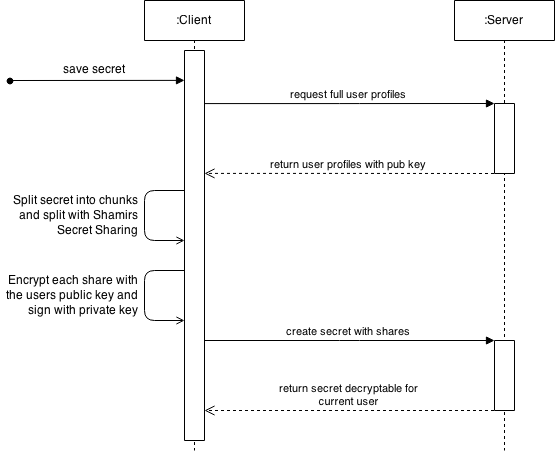
\includegraphics[scale=0.65]{pictures/create_secret_sequence_diagram.png}
  \centering
  \caption{Creating a secret}
  \label{fig:creating_a_secret}
\end{figure}
